\documentclass{article}

\usepackage[x11names]{xcolor}
\usepackage{pgfplots}

\begin{document}



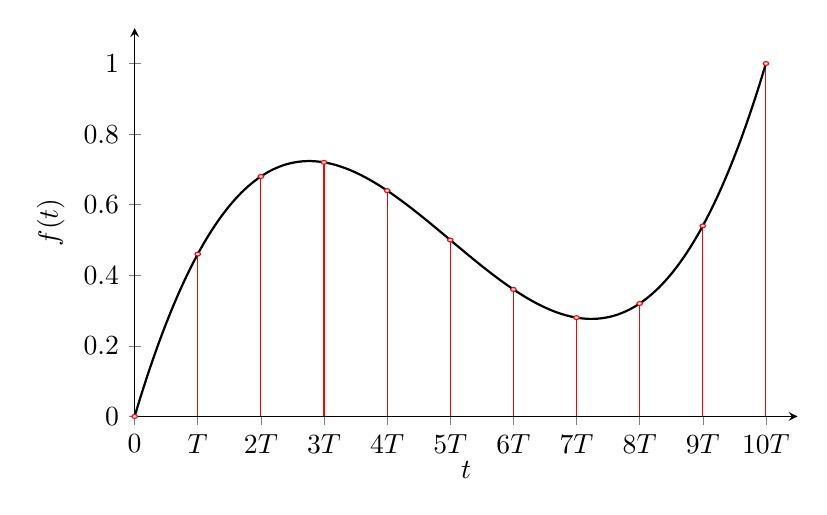
\begin{tikzpicture}
\begin{axis}[
	width=10cm,
	yscale=0.7,
    axis lines=left,
    clip=false,
    axis on top,
	ybar=1pt,
	bar width=0pt,
	/pgf/declare function={f=(-15*(x-5)+(x-5)^3+50)/100;},
	xlabel=$t$,
	ylabel=$f(t)$,
	xtick={0,1,2,3,4,5,6,7,8,9,10},
	xticklabels={$0$,$T$,$2T$,$3T$,$4T$,$5T$,$6T$,$7T$,$8T$,$9T$,$10T$},
	xmax=10.5,
	ymax=1.1
    ]

\addplot [draw=red, fill=red!10,, samples=11, domain=0:10, mark=*, mark size=1pt] {f}\closedcycle;

\addplot[smooth, thick,domain=0:10,samples=101]{f};

\end{axis}
\end{tikzpicture}

\begin{equation}
f^*(t) = \sum_{n=0}^{\infty} f(t)\delta(t-nT)
\end{equation}
\end{document}
